% GNUPLOT: LaTeX picture with Postscript
\begingroup
  \fontfamily{Times-Roman}%
  \selectfont
  \makeatletter
  \providecommand\color[2][]{%
    \GenericError{(gnuplot) \space\space\space\@spaces}{%
      Package color not loaded in conjunction with
      terminal option `colourtext'%
    }{See the gnuplot documentation for explanation.%
    }{Either use 'blacktext' in gnuplot or load the package
      color.sty in LaTeX.}%
    \renewcommand\color[2][]{}%
  }%
  \providecommand\includegraphics[2][]{%
    \GenericError{(gnuplot) \space\space\space\@spaces}{%
      Package graphicx or graphics not loaded%
    }{See the gnuplot documentation for explanation.%
    }{The gnuplot epslatex terminal needs graphicx.sty or graphics.sty.}%
    \renewcommand\includegraphics[2][]{}%
  }%
  \providecommand\rotatebox[2]{#2}%
  \@ifundefined{ifGPcolor}{%
    \newif\ifGPcolor
    \GPcolortrue
  }{}%
  \@ifundefined{ifGPblacktext}{%
    \newif\ifGPblacktext
    \GPblacktexttrue
  }{}%
  % define a \g@addto@macro without @ in the name:
  \let\gplgaddtomacro\g@addto@macro
  % define empty templates for all commands taking text:
  \gdef\gplbacktext{}%
  \gdef\gplfronttext{}%
  \makeatother
  \ifGPblacktext
    % no textcolor at all
    \def\colorrgb#1{}%
    \def\colorgray#1{}%
  \else
    % gray or color?
    \ifGPcolor
      \def\colorrgb#1{\color[rgb]{#1}}%
      \def\colorgray#1{\color[gray]{#1}}%
      \expandafter\def\csname LTw\endcsname{\color{white}}%
      \expandafter\def\csname LTb\endcsname{\color{black}}%
      \expandafter\def\csname LTa\endcsname{\color{black}}%
      \expandafter\def\csname LT0\endcsname{\color[rgb]{1,0,0}}%
      \expandafter\def\csname LT1\endcsname{\color[rgb]{0,1,0}}%
      \expandafter\def\csname LT2\endcsname{\color[rgb]{0,0,1}}%
      \expandafter\def\csname LT3\endcsname{\color[rgb]{1,0,1}}%
      \expandafter\def\csname LT4\endcsname{\color[rgb]{0,1,1}}%
      \expandafter\def\csname LT5\endcsname{\color[rgb]{1,1,0}}%
      \expandafter\def\csname LT6\endcsname{\color[rgb]{0,0,0}}%
      \expandafter\def\csname LT7\endcsname{\color[rgb]{1,0.3,0}}%
      \expandafter\def\csname LT8\endcsname{\color[rgb]{0.5,0.5,0.5}}%
    \else
      % gray
      \def\colorrgb#1{\color{black}}%
      \def\colorgray#1{\color[gray]{#1}}%
      \expandafter\def\csname LTw\endcsname{\color{white}}%
      \expandafter\def\csname LTb\endcsname{\color{black}}%
      \expandafter\def\csname LTa\endcsname{\color{black}}%
      \expandafter\def\csname LT0\endcsname{\color{black}}%
      \expandafter\def\csname LT1\endcsname{\color{black}}%
      \expandafter\def\csname LT2\endcsname{\color{black}}%
      \expandafter\def\csname LT3\endcsname{\color{black}}%
      \expandafter\def\csname LT4\endcsname{\color{black}}%
      \expandafter\def\csname LT5\endcsname{\color{black}}%
      \expandafter\def\csname LT6\endcsname{\color{black}}%
      \expandafter\def\csname LT7\endcsname{\color{black}}%
      \expandafter\def\csname LT8\endcsname{\color{black}}%
    \fi
  \fi
    \setlength{\unitlength}{0.0500bp}%
    \ifx\gptboxheight\undefined%
      \newlength{\gptboxheight}%
      \newlength{\gptboxwidth}%
      \newsavebox{\gptboxtext}%
    \fi%
    \setlength{\fboxrule}{0.5pt}%
    \setlength{\fboxsep}{1pt}%
\begin{picture}(4896.00,3024.00)%
    \gplgaddtomacro\gplbacktext{%
      \csname LTb\endcsname%
      \put(490,456){\makebox(0,0)[r]{\strut{}$0$}}%
      \csname LTb\endcsname%
      \put(490,970){\makebox(0,0)[r]{\strut{}$0.2$}}%
      \csname LTb\endcsname%
      \put(490,1483){\makebox(0,0)[r]{\strut{}$0.4$}}%
      \csname LTb\endcsname%
      \put(490,1997){\makebox(0,0)[r]{\strut{}$0.6$}}%
      \csname LTb\endcsname%
      \put(490,2510){\makebox(0,0)[r]{\strut{}$0.8$}}%
      \csname LTb\endcsname%
      \put(570,266){\makebox(0,0){\strut{}$0$}}%
      \csname LTb\endcsname%
      \put(1111,266){\makebox(0,0){\strut{}$8$}}%
      \csname LTb\endcsname%
      \put(1651,266){\makebox(0,0){\strut{}$16$}}%
      \csname LTb\endcsname%
      \put(2192,266){\makebox(0,0){\strut{}$24$}}%
      \csname LTb\endcsname%
      \put(2733,266){\makebox(0,0){\strut{}$32$}}%
      \csname LTb\endcsname%
      \put(3273,266){\makebox(0,0){\strut{}$40$}}%
      \csname LTb\endcsname%
      \put(3814,266){\makebox(0,0){\strut{}$48$}}%
      \csname LTb\endcsname%
      \put(4354,266){\makebox(0,0){\strut{}$56$}}%
      \csname LTb\endcsname%
      \put(4895,266){\makebox(0,0){\strut{}$64$}}%
    }%
    \gplgaddtomacro\gplfronttext{%
      \csname LTb\endcsname%
      \put(19,1502){\rotatebox{-270}{\makebox(0,0){\strut{}\JaccardRand{\secretsSetSize}}}}%
      \put(2732,95){\makebox(0,0){\strut{}$\log_2{\secretsSetSize}$}}%
      \csname LTb\endcsname%
      \put(877,2866){\makebox(0,0)[l]{\strut{}v3.18-1run}}%
      \csname LTb\endcsname%
      \put(877,2676){\makebox(0,0)[l]{\strut{}v3.18-patched}}%
      \csname LTb\endcsname%
      \put(2422,2866){\makebox(0,0)[l]{\strut{}v3.18-2run}}%
      \csname LTb\endcsname%
      \put(3450,2676){\makebox(0,0)[l]{\strut{}v3.18-rmCounter}}%
      \csname LTb\endcsname%
      \put(3967,2866){\makebox(0,0)[l]{\strut{}v3.18-3run}}%
    }%
    \gplgaddtomacro\gplbacktext{%
      \csname LTb\endcsname%
      \put(1121,907){\makebox(0,0)[r]{\strut{}0}}%
      \put(1121,1310){\makebox(0,0)[r]{\strut{}0.2}}%
      \put(1121,1713){\makebox(0,0)[r]{\strut{}0.4}}%
      \put(1121,2116){\makebox(0,0)[r]{\strut{}0.6}}%
      \put(1224,770){\makebox(0,0){\strut{}0}}%
      \put(1591,770){\makebox(0,0){\strut{}1}}%
      \put(1958,770){\makebox(0,0){\strut{}2}}%
      \put(2325,770){\makebox(0,0){\strut{}3}}%
      \put(2692,770){\makebox(0,0){\strut{}4}}%
      \put(3059,770){\makebox(0,0){\strut{}5}}%
      \put(3426,770){\makebox(0,0){\strut{}6}}%
      \put(3793,770){\makebox(0,0){\strut{}7}}%
      \put(4160,770){\makebox(0,0){\strut{}8}}%
    }%
    \gplgaddtomacro\gplfronttext{%
    }%
    \gplbacktext
    \put(0,0){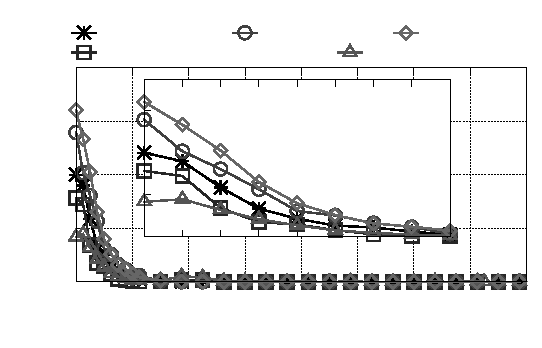
\includegraphics{linux-other}}%
    \gplfronttext
  \end{picture}%
\endgroup
